\documentclass[conference]{IEEEtran}
\usepackage{times}
\usepackage{multirow}
\usepackage{amsmath}
\usepackage{amsopn}
\usepackage{color}
\DeclareMathOperator*{\argmin}{\arg\!\min} 
\DeclareMathOperator*{\argmax}{\arg\!\max} 

\usepackage{graphicx}
\usepackage{caption}
\usepackage{subcaption}
% numbers option provides compact numerical references in the text. 
\usepackage[numbers]{natbib}
\usepackage{multicol}
\usepackage[bookmarks=true]{hyperref}

\newcommand{\sw}[1]{\textcolor{red}{SW: #1}}

\pdfinfo{
   /Author (Homer Simpson)
   /Title  (Robots: Our new overlords)
   /CreationDate (D:20101201120000)
   /Subject (Robots)
   /Keywords (Robots;Overlords)
}

\begin{document}

% paper title
\title{Inverse Reinforcement Learning from Failure}

% You will get a Paper-ID when submitting a pdf file to the conference system
%\author{Kyriacos Shiarlis, Jo\~{a}o Messias, Maarten van Someren, and Shimon 
%Whiteson}

\author{\authorblockN{Kyriacos Shiarlis, Jo\~{a}o Messias, Maarten van Someren, 
and Shimon Whiteson}
\authorblockA{University of Amsterdam\\
%Georgia Institute of Technology\\
%Amsterdam, Netherlands\\
Email: \{K.C.Shiarlis, jmessias, M.W.vanSomeren, S.A.Whiteson\}@uva.nl}
%\and
%\authorblockN{Homer Simpson}
%\authorblockA{Twentieth Century Fox\\
%Springfield, USA\\
%Email: homer@thesimpsons.com}
%\and
%\authorblockN{James Kirk\\ and Montgomery Scott}
%\authorblockA{Starfleet Academy\\
%San Francisco, California 96678-2391\\
%Telephone: (800) 555--1212\\
%Fax: (888) 555--1212}}
}

% avoiding spaces at the end of the author lines is not a problem with
% conference papers because we don't use \thanks or \IEEEmembership


% for over three affiliations, or if they all won't fit within the width
% of the page, use this alternative format:
% 
%\author{\authorblockN{Michael Shell\authorrefmark{1},
%Homer Simpson\authorrefmark{2},
%James Kirk\authorrefmark{3}, 
%Montgomery Scott\authorrefmark{3} and
%Eldon Tyrell\authorrefmark{4}}
%\authorblockA{\authorrefmark{1}School of Electrical and Computer Engineering\\
%Georgia Institute of Technology,
%Atlanta, Georgia 30332--0250\\ Email: mshell@ece.gatech.edu}
%\authorblockA{\authorrefmark{2}Twentieth Century Fox, Springfield, USA\\
%Email: homer@thesimpsons.com}
%\authorblockA{\authorrefmark{3}Starfleet Academy, San Francisco, California 96678-2391\\
%Telephone: (800) 555--1212, Fax: (888) 555--1212}
%\authorblockA{\authorrefmark{4}Tyrell Inc., 123 Replicant Street, Los Angeles, California 90210--4321}}


\maketitle

\begin{abstract}
In this paper, we approach the problem of Inverse Reinforcement Learning (IRL) from a rather different perspective. Instead of trying to only mimic an expert as in traditional IRL, we present a method that can utilise information from failed or bad demonstrations of a task. To this end, we propose a new IRL algorithm that extends the state-of-the-art method of Maximum Causal Entropy Inverse Reinforcement Learning. Furthermore, we present experimental results showing that our method can converge faster and is more sample efficient than its original counterpart, at no extra computational cost. 
\end{abstract}

\IEEEpeerreviewmaketitle

\section{Introduction}
In Inverse Reinforcement Learning (IRL) \cite{ng2000algorithms}, an \emph{apprentice} aims to learn a policy for acting in an environment modelled by a Markov Decision Process (MDP) for which the reward function is not available, but samples from the policy of an \emph{expert} performing the task are given instead. An IRL algorithm tries to find a reward function that leads the apprentice to exhibit behaviour that is similar to the expert's, and that generalises well to situations for which expert data is not available. %The IRL formulation is particularly appealing in MDPs for which the actual reward function is difficult to define explicitly, but examples of correct behaviour can be generated instead. For this exact reason 
IRL methods have been applied to simulated car driving \cite{abbeel2004apprenticeship} and socially appropriate navigation \cite{henry2010learning,vasquez2014inverse}. Existing IRL methods leverage concepts from the wider Machine Learning community, such as maximum entropy \cite{ziebart2008maximum} and Bayesian formulations \cite{ramachandran2007bayesian}, structured classification \cite{ratliff2006maximum}, boosting \cite{ratliff2007boosting} and Gaussian processes \cite{levine2011nonlinear}.

Existing IRL algorithms learn only from successful trials, i.e., from data gathered by having an expert performing the task well. This is consistent with the main motivation of IRL since it allows learning in tasks where the reward cannot be trivially hardcoded.  For example, the cost function that allows an agent to perform complicated manoeuvres while flying a helicopter cannot be trivially determined, but examples of the task can be easily obtained from an expert.

%
%Existing IRL algorithms learn only from successful trials, i.e., from data gathered by having an expert performing the task well.  This is consistent with one of the main motivations for IRL, that it allows learning in tasks in which it is too dangerous for an agent to explore.  For example, since it is not safe to let a learning agent fly (and probably crash) a helicopter while it is learning, data is first gathered by an expert pilot whom the agent then learns to mimic. 


However, in many realistic scenarios, failed trials are also readily available.  Consider for example tasks such as driving a car.  Since humans also learn this task by trial and error, demonstrations of both successful and failed behaviour are available. Moreover, although hand-coding a reward function for this task would be infeasible, labelling each trial as successful or failed is straightforward.

In this paper, we present the first IRL algorithm that can learn from both successful and failed demonstrations.  In doing so, we address a key difficulty in IRL: the problem is typically under-constrained since many reward functions are consistent with the expert's behaviour.  By making use of failed trials, our method reduces this ambiguity, resulting in faster and better learning.

To derive an IRL algorithm for learning from failure, we start from the state-of-the-art method of Maximum Causal Entropy Inverse Reinforcement Learning \cite{ziebart2008maximum}.  This approach starts by formulating a constrained optimization problem that seeks a reward function that yields trajectories through state-action space consistent with those of the expert.  We formulate a new optimization problem with additional constraints that require the resulting trajectories to also be maximally different from the failed trajectories. Then, by applying the method of Lagrangian multipliers, we produce our new method, which learns from both successful and failed trajectories.
	Our empirical results show that utilising failed trials can result in learning  a reward function that is closer to that of the expert, in fewer iterations.



% Despite its appealing applications and encouraging research the IRL framework still suffers from a number of important theoretical and practical drawbacks. Firstly, because of their iterative nature most known methods require solving an MDP under the current reward before an update. For large state spaces, Markov decision processes becomes prohibitive to evaluate once, let alone a number of times. Secondly, most algorithms are non-convex in nature especially if the dynamics of the system are non-deterministic and ill posed how do I make the differentiation? More practical issues include generalisation, if the observed expert's behaviour is too limited, it is very hard to generalise to new parts of the state space, especially if this is too large. In addition, since the expert can be expected to avoid punishing states, information about the reward in these states reaches us only implicitly, making generalisation of the reward function an even harder task. \\

% We present the first step towards allowing IRL algorithms to leverage a wider variety of data to learn faster and generalise better. Specifically we consider the case where appart from
% an Expert dataset we have access to a dataset of behaviour that should be avoided at all costs. Our algorithm tries to approach the expert behaviour at while avoiding the failed trajectories.

% This altered view of IRL emerges from the basic principle that governs most IRL algorithms. Because the observed data is assumed to be coming from an Expert, IRL tries to make the value of the observed trajectories optimal by tweeking the reward function in an intelligent way, most commonly by gradient (or subgradient) descent. We can imagine however that we observe a certain trajectory in the state space and we have access to an annotator that can tell us to what \emph{degree} the observe behaviour is optimal. If for example we observe the worst possible behaviour, then we can possibly demand from our algorithm to \emph{minimise} value for those trajectories when generated by the apprentice. Importanly, this view preserves the main motivation for IRL which is that the reward function for each state-action pair need not be hardcoded, while \emph{extending} the scope from which demonstrations can be considered useful to learning. In addition, by exploiting the information contained within, for example, failed trajectories, we gain access to more explicit information about the nature of the reward at certain areas of the state-space that the expert could only implicitly provide. This provides additional constraints to combat the aforementioned illposition of IRL and allow's us to build reward functions that are more likely to generalise to unseen situations. Finally such a framework would allow the designer to inject prior knowledge into the learning process in a principled manner, without the need for complex prior distributions and extra computational cost. If we are previously aware of parts of the state-space that should have a very negative reward, we can (assuming the dynamics are known) simulate data of the agent acting in an environment where large rewards are given for reaching unwanted states. Feeding our generated data along with that of the expert into our extended IRL algorithm would allow the apprentice to imitate the expert while learning a reward function that takes into account our domain knowledge.



\section{Method}
In \cite{ziebart2010modelingthesis} Ziebart proposes an IRL method based on the principle of Maximum Causal Entropy.  The main idea is to find a stochastic policy $\pi(a,s)$ that maximises the causal entropy $H(\mathbf{A}^T||\mathbf{S}^T)$ of all actions $\mathbf{A}^T$ taken in a decision time horizon $T$, given the visited states $\mathbf{S}^T$, while constrained to match certain statistics from the expert dataset $\mathcal{D}$. These statistics are called the \emph{empirical feature expectations} $\widetilde{\Phi}_{\mathcal{D}}$. This task is formalized as a constrained convex optimization problem which is then addressed using the method of Lagrangian multipliers.  
%
Each assignment of these multipliers defines a specific reward function, which is optimized as follows. A policy is found under the current reward function using a Bellman equation with a softmax operator instead of a maximum.  The feature expectations of the model are then calculated from $\mathcal{D}$. Finally, the multipliers are updated based on the comparison between the empirical and model feature expectations.

Our method extends this approach in two key ways. First, we relax the constraint that the model should exactly match $\widetilde{\Phi}_{\mathcal{D}}$ by introducing slack variables ($\zeta^+$ and $\zeta^-$).  Second, we introduce new constraints that enforce dissimilarity between the model and $\widetilde{\Phi}_{\mathcal{D}_b}$, the feature expectations of the failed demonstrations. This is done through a second set of slacks ($\alpha^+$ and $\alpha^-$). The resulting constrained optimization problem is:
	
	\begin{equation*}
	\argmax_{\pi(a,s),\alpha^+_k ,\alpha^-_k ,\zeta^+_k, \zeta^-_k} H(\mathbf{A}^T||\mathbf{S}^T) - \sum_k\big(C(\zeta^+_k + \zeta^-_k)  -D(\alpha^+_k  \alpha^-_k)\big)
\end{equation*}
Subject to:
\begin{equation*}
  \widetilde{\Phi}_{\mathcal{D},k}-\Phi_{\pi,s_0,k}   = \zeta^+_k  - \zeta^-_k \quad \forall k, \label{eq:good_ineq}
\end{equation*}
\begin{equation*}
	\widetilde{\Phi}_{\mathcal{D}_b,k}-\Phi_{\pi,s_0,k}  = \alpha^+_k-\alpha^-_k \quad \forall k, \label{eq:bad_ineq}
\end{equation*}
\begin{equation*}
	-\zeta^+_k \leq 0 \quad \text{and} \quad -\zeta^-_k \leq 0 \quad \forall k,
\end{equation*}
\begin{equation*}
	-\alpha^+_k \leq 0 \quad \text{and} \quad -\alpha^-_k \leq 0 \quad \forall k,
\end{equation*}
\begin{equation*}
	\alpha^-_k \alpha^+_k = 0 \quad \forall k,  \label{eq:quadratic}
\end{equation*}
\begin{equation*}
\sum_aP(a|s)  = 1 \quad \forall s,   \quad \text{and} \quad P(a|s)  > 0 \quad \forall s,a.  
\end{equation*}
Where $s$ and $a$ are the individual states and actions considered in our MDP model. D and C are constants that act on the slacks $\alpha$ and $\zeta$ respectively and determine how much we value maximising or minimising them. The optimisation is handled very much like the original algorithm, using Lagrangian multipliers. The Lagrangian is first maximised with respect to the variables in the objective function to obtain a Dual. We then update the Lagrange multipliers by taking a step in the direction that maximises this Dual.

\section{Results \& Discussion}

We compared the performance of our method to Ziebart's original IRL method on a simulated robot control task that requires avoiding moving obstacles.  In particular, the robot aims to reach a target state (T) of very high reward,
while avoiding some states of negative reward (N). The (N) states change throughout time.
 
To set up the experiments, we defined two reward functions, $R_e$ and $R_t$, both of which are unknown to the learning algorithms.  $R_e$, the expert's reward function, is the true reward function while $R_t$ is the reward function used by a \emph{taboo agent} that generates the failed trajectories. Specifically the taboo agent attempts to approach the (N) states rather than avoid them, and has no knowledge of the target.  Using these reward functions, we generate the feature expectations $\widetilde{\Phi}_{\mathcal{D},k}$ and $\widetilde{\Phi}_{\mathcal{D}_b,k}$ by allowing agents using soft-optimal policies w.r.t.\ $R_e$ and $R_t$ to start from an initial state distribution $b_{0,train}$ and proceed for $T$ timesteps.  Based on this data, we train two apprentices, one using Ziebart's method and one using ours.  Finally, we evaluate performance on a test distribution of initial states $b_{0,test}$. 

% The evaluation is done based on three metrics namely:

% 		We evaluate the toy problem based on three initial criteria:
% 			\begin{itemize}
% 				\item The value accumulated by the apprentice in T timesteps starting from $b_{0,test}$ when evaluated on the experts reward function, $R_e$. If the apprentice achieves similar Value accumulation as the expert, it means that the trajectories executed by the two agent's are similar.

% 				\item The value accumulated by the apprentice in N timesteps from a test initial state distribution $b_{0,test}$ when evaluated on the initial taboo agents reward function $R_t$. The less Value is accumulated here, the better since we want to perform badly on the taboo-agents reward function.
% 				\end{itemize}

Figure \ref{fig:res}a shows the average value, with respect to $R_e$, of the policies found by the two methods, at each iteration.  Our approach is able to ultimately match the value of the expert's policy while Ziebart's method plateaus lower. Figure \ref{fig:res}b also shows the average value of the two methods with respect to $R_t$.  In this case, lower values are better as they correspond to performing badly on a bad reward function.  The results indicate that our method does a better job of minimizing value with respect to $R_t$ than Ziebart's method.  This figure also shows the performance of the expert's policy with respect to $R_t$ (green). Unlike Ziebart's method, our method is able to accumulate less value with respect to $R_t$ than the expert's policy.

\begin{figure}[t]
  \hspace{-5pt}
  \begin{subfigure}{0.22\textwidth}

    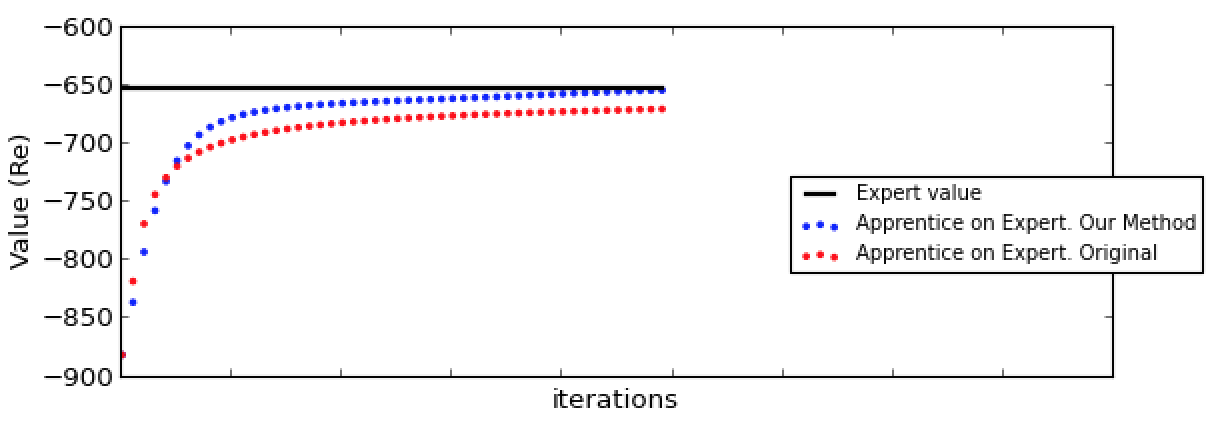
\includegraphics[scale = 0.22]{figures/resa.png}
    \caption{Expert Reward Function}
    \label{fig:res_a}
  \end{subfigure}
  \hspace{25pt}
  \begin{subfigure}{0.22\textwidth}
	  
    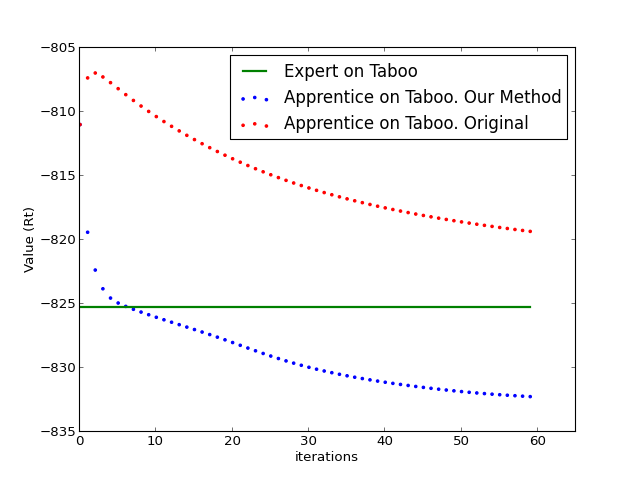
\includegraphics[scale = 0.22]{figures/resb.png}
        \caption{Taboo Reward Function}
    \label{fig:res_b}
\end{subfigure}
  \caption{\small{\textit{Results from the moving obstacle avoidance task.  Learning from failure (blue) yields behavior that is more similar to that of the expert and more dissimilar to that of the taboo agent than Ziebart's IRL method (red).}} }
  \label{fig:res}
\vspace{-4mm}
\end{figure}


These results demonstrate that taking into account failed demonstrations of a task can allow an apprentice to generalise better to new initial states and learn in fewer iterations than previously possible.  In the future, we aim to apply this method to more realistic scenarios such as those involving real robots. We also hope to examine how the similarity between the expert and taboo datasets affect the ability to learn. Finally, we would like to extend our modifications to other popular IRL algorithms.

%Proof of concept that failed trajectories contain valuable information for learning in many fronts. 
%Further work includes:
%\begin{itemize}
%	\item Tackling problems of having very similar data from expert and non expert.
%	\item Applying concept to other methods that might require different treatment.
%\end{itemize}
%
%
%\section{RSS citations}
%
%Please make sure to include \verb!natbib.sty! and to use the
%\verb!plainnat.bst! bibliography style. \verb!natbib! provides additional
%citation commands, most usefully \verb!\citet!. For example, rather than the
%awkward construction 
%
%{\small
%\begin{verbatim}
%\cite{kalman1960new} demonstrated...
%\end{verbatim}
%}
%
%\noindent
%rendered as ``\cite{kalman1960new} demonstrated...,''
%or the
%inconvenient 
%
%{\small
%\begin{verbatim}
%Kalman \cite{kalman1960new} 
%demonstrated...
%\end{verbatim}
%}
%
%\noindent
%rendered as 
%``Kalman \cite{kalman1960new} demonstrated...'', 
%one can
%write 
%
%{\small
%\begin{verbatim}
%\citet{kalman1960new} demonstrated... 
%\end{verbatim}
%}
%\noindent
%which renders as ``\citet{kalman1960new} demonstrated...'' and is 
%both easy to write and much easier to read.
%  
%\subsection{RSS Hyperlinks}
%
%This year, we would like to use the ability of PDF viewers to interpret
%hyperlinks, specifically to allow each reference in the bibliography to be a
%link to an online version of the reference. 
%As an example, if you were to cite ``Passive Dynamic Walking''
%\cite{McGeer01041990}, the entry in the bibtex would read:
%
%{\small
%\begin{verbatim}
%@article{McGeer01041990,
%  author = {McGeer, Tad}, 
%  title = {\href{http://ijr.sagepub.com/content/9/2/62.abstract}{Passive Dynamic Walking}}, 
%  volume = {9}, 
%  number = {2}, 
%  pages = {62-82}, 
%  year = {1990}, 
%  doi = {10.1177/027836499000900206}, 
%  URL = {http://ijr.sagepub.com/content/9/2/62.abstract}, 
%  eprint = {http://ijr.sagepub.com/content/9/2/62.full.pdf+html}, 
%  journal = {The International Journal of Robotics Research}
%}
%\end{verbatim}
%}
%\noindent
%and the entry in the compiled PDF would look like:
%
%\def\tmplabel#1{[#1]}
%
%\begin{enumerate}
%\item[\tmplabel{1}] Tad McGeer. \href{http://ijr.sagepub.com/content/9/2/62.abstract}{Passive Dynamic
%Walking}. {\em The International Journal of Robotics Research}, 9(2):62--82,
%1990.
%\end{enumerate}
%%
%where the title of the article is a link that takes you to the article on IJRR's website. 
%
%
%Linking cited articles will not always be possible, especially for
%older articles. There are also often several versions of papers
%online: authors are free to decide what to use as the link destination
%yet we strongly encourage to link to archival or publisher sites
%(such as IEEE Xplore or Sage Journals).  We encourage all authors to use this feature to
%the extent possible.
%\section*{Acknowledgments}

%% Use plainnat to work nicely with natbib. 

\bibliographystyle{plainnat}
\bibliography{references}

\end{document}


